%----------------------------------------------------------------------
% COMPUTATIONAL PHYSICS - PROJECT 1
% SEMICLASSICAL QUANTIZATION OF MOLECULAR VIBRATIONS
%----------------------------------------------------------------------

\documentclass[a4paper]{IEEEtran} 
\usepackage{amssymb}
\usepackage{moreverb}
\usepackage[cmex10]{amsmath} 
\usepackage{cite} 
\usepackage{graphicx} 
\usepackage[colorlinks=false, hidelinks]{hyperref} 

\usepackage{listings} 
\usepackage{color} 
\usepackage{xcolor}  
\usepackage{microtype} 
\usepackage{microtype} 
\usepackage{inconsolata} 
\usepackage[framemethod=TikZ]{mdframed} 
\usepackage{alltt}
\usepackage{sverb} 
\usepackage{verbatim} 
\usepackage{pifont} 
\usepackage{alltt} 
\usepackage{helvet} 

%----------------------------------------------------------------------
% CODE LISTING SETTINGS
%----------------------------------------------------------------------

\lstset{language=fortran,
        %basicstyle=\footnotesize\ttfamily, 
        basicstyle=\small\ttfamily,
        columns=fullflexible, 
        %title=\lstname, 
        numbers=left, stringstyle=\texttt, 
        numberstyle={\tiny\texttt}, 
        keywordstyle=\color{blue}, 
        commentstyle=\color{darkgreen}, 
        stringstyle=\color{purple} } 


\mdfsetup{skipabove=\topskip, skipbelow=\topskip} 

\definecolor{codebg}{rgb}{0.99,0.99,0.99}

\global\mdfdefinestyle{code}{%
    frametitlerule=true,%
    frametitlefont=\small\bfseries\ttfamily,%
    frametitlebackgroundcolor=lightgray,%
    backgroundcolor=codebg,%
    linecolor=gray, linewidth=0.5pt,%
    leftmargin=0.5cm, rightmargin=0.5cm,%
    roundcorner=2pt,%
    innerleftmargin=5pt
}

\global\mdfdefinestyle{code2}{%
    topline=false,%
    bottomline=false,%
    leftline=true,%
    rightline=false,%
    backgroundcolor=codebg,%
    linecolor=gray, linewidth=0.5pt,%
    leftmargin=0.0cm, rightmargin=0.0cm,%
    innerleftmargin=1pt
}

\newcommand{\showcode}[1]{\begin{mdframed}[style=code] %
                            \lstinputlisting{#1}% 
                          \end{mdframed}% 
}

\newcommand{\showsmallcode}[1]{\begin{mdframed}[style=code2] %
        \lstinputlisting[basicstyle=\ttfamily\tiny]{#1}% 
                          \end{mdframed}% 
}




%----------------------------------------------------------------------
% IEEE SETTINGS
%----------------------------------------------------------------------

\interdisplaylinepenalty=2500
\setlength{\IEEEilabelindent}{\IEEEilabelindentB}

%\markboth{630--364 Computational Physics}{} 
\markboth{Semi-Classical Quantization of Molecular Vibrations. Michael Papasimeon. 1997}{} 

%----------------------------------------------------------------------
% BEGIN DOCUMENT
%----------------------------------------------------------------------

\title{Semi-Classical Quantization of Molecular Vibrations}
\author{Michael Papasimeon\\ 12 August 1997} % \\
\date{August 12, 1997}

%----------------------------------------------------------------------
% BEGIN DOCUMENT
%----------------------------------------------------------------------

\begin{document}
\maketitle
%\thispagestyle{plain} 

\begin{abstract}
This paper was written for an introductory undegraduate class in computational
physics in 1997. It focuses on basic computational/numerical techniques
for quadrature and root finding. It then applies these techniques to finding 
the energy levels of molecular hydrogen $H_2$ using a semi-classical quantization 
approach. The source code listings in \textsc{Fortran77} can be found in the appendices.
\end{abstract} 

%----------------------------------------------------------------------
% QUADRATURE
%----------------------------------------------------------------------

\section{Quadrature}

\subsection{Aims}

      \IEEEPARstart{T}{he}
      main aim is to write a FORTRAN program to numerically integrate 
      the integral:
      \begin{equation}
            \label{quadint}
            \int_{0}^{1} \frac{\ln(1+x)}{x} dx = \frac{\pi^{2}}{12}
      \end{equation}
      \begin{itemize}
            \item using the Trapezoidal rule,
            \item using Simpson's method,
            \item and to investigate the accuracy of both the
                  Trapezoidal rule and Simpson's method for different
                  step sizes.
      \end{itemize}

\subsection{Procedure}

    A FORTRAN program was written (\verb+quad.f+, source code in Appendix A),
    which implemented both the Trapezoidal and Simpson's rules for the 
    quadrature of equation~\ref{quadint}. The program calls the
    functions to calculate the integral a number of times each with a
    diiferent number of divisions $n$, and hence step size $h$. Both
    the Trapezoidal and Simpson's rules are evaluated at number of
    divisions 
    starting from $n=10$ to $n=10^6$, with each new evaluation
    increasing by a single order of magnitude. This allows the
    investigation of the accuracy of the different techniques as the
    number of divisions increases.

    The error is calculated is the absolute error:
        \[ Error = \mathrm{abs}(Result - Answer) \]
    where Result is the value produced by the numerical technique and
    $Answer$, is the analytic solution to the integral known to
    be $\frac{\pi^{2}}{12} \simeq 0.822467033$.

    Since the integrand is not defined at $x=0$, the FORTRAN function
    used to evaluate this returns a value of $1.0$ when $x=0$, this is
    because
        \[ \lim_{x \rightarrow 0} \frac{\ln(1+x)}{x} = 1 \].


\subsection{Results}

    \subsubsection{Trapezoidal Rule}
    The output from the program \verb+quad.f+ using the Trapezoidal
    rule is shown below in in Table~\ref{tbl:trapezoidal} 

    \begin{table}[h] 
      \caption{Results of using Trapezoidal rule.} 
      \label{tbl:trapezoidal} 
      \begin{center}
      \begin{tabular}{|r|r|r|r|} \hline
           $n$  &         $h$   &     $Result$ &   $Error$ \\ 
       \hline
       \hline
            10  & .1000000000   &.8227225585   &.255525E-03 \\
           100  & .0100000000   &.8224695905   &.255709E-05 \\
          1000  & .0010000000   &.8224670590   &.255711E-07 \\
         10000  & .0001000000   &.8224670337   &.255709E-09 \\
        100000  & .0000100000   &.8224670334   &.255251E-11 \\
       1000000  & .0000010000   &.8224670334   &.263123E-13 \\ \hline
       \end{tabular}
       \end{center} 
    \end{table} 

    \subsubsection{Simpson's Rule}
    The output from the program \verb+quad.f+ using Simpson's rule is
    shown below in Table~\ref{tbl:simpsons}.

    \begin{table}[h] 
    \caption{Results using Simpson's rule.} 
    \label{tbl:simpsons} 
    \begin{center}
    \begin{tabular}{|r|r|r|r|} \hline
            $n$   &          $h$  &      $Result$ &        $Error$ \\
    \hline 
    \hline
           10   &.1000000000   &.8224677660   &.732614E-06 \\
          100   &.0100000000   &.8224670335   &.744940E-10 \\
         1000   &.0010000000   &.8224670334   &.799361E-14 \\
        10000   &.0001000000   &.8224670334   &.310862E-14 \\
       100000   &.0000100000   &.8224670334   &.310862E-14 \\
      1000000   &.0000010000   &.8224670334   &.643929E-14 \\ \hline
    \end{tabular}
    \end{center}
    \end{table} 
  
\subsection{Discussion}

    Looking at the results for the Trapezoidal rule calculations 
    in Table 1, we see that as we increase the
    number of divisions $n$ by one order of magnitude, the error
    decreases by 2 orders. Therefore, we see that when using the
    Trapezoidal rule for quadrature, the error is of order $O(n^2)$, as 
    expected.

    Making a comparison with the results for the Simpson's rule
    calculations shown in Table 2, we see that that as the number of
    divisions $n$ is increased by an order of magnitude, the error
    decreases by 4 orders. Therefore, when using Simpson's rule, the
    error is of order $O(n^4)$. 
    The only problem is that the magnitude of the error stops decreasing
    after n = 10000. The most likely explanation for this is that we
    have reached the floating point limit on the number of decimal
    places which the computer which ran the program can handle.

    Therefore we see that that Simpson's rule is more accurate than the
    trapezoidal rule for quadrature.

%----------------------------------------------------------------------
% ROOT FINDING
%----------------------------------------------------------------------

\section{Root Finding}

\subsection{Aims}

    The main aim is to write a FORTRAN program which makes use of the
    false position method to calculate the non zero root of the 
    equation
    \begin{equation}
        \label{false}
        \int_{0}^{x} t^2 dt = x
    \end{equation}
    and to compare with the analytic solution. The program will make use
    of the Simpson's rule to evaluate the integral.

\subsection*{Procedure}
    Firstly equation~\ref{false} must be solved analytically.
    \begin{eqnarray}
        \int_{0}^{x} t^2 dt         & = & x \nonumber \\
        \left[\frac{t^3}{2}\right]_{0}^{x} - x & = & 0 \nonumber \\
        \frac{x^3}{3} - x & = & 0 \nonumber \\
        x\left(\frac{x^2}{3} - 1\right) & = & 0 \nonumber 
    \end{eqnarray}
    Therefore equation~\ref{false} has three roots
        \[ x = 0, \pm\sqrt{3} \]
    We are interested in finding the positive root,
    $x = +\sqrt{3} \simeq 1.732050808$, of equation~\ref{false} numerically.

    The procedure involved writing a FORTRAN program to find the roots
    of the equation
        \[ \int_{0}^{x} t^2 dt -x = 0 \].
    The algorithm used to find the root of this equation was the false
    position method. Simpson's rule was also used in the program to
    evaluate the integral in the equation.

    The program outputs a table of results, with varying number of
    divisions $n$ for the Simpson rule calculations and varying
    $Tolerance$ for the false position method. The values of $n$ range
    from $n = 10$ to $n = 10^7$ with each one being an order of
    magnitude of the previous value. The value for the tolerance of the
    false position algorithm is simply $1/n$.

    The source code for the program \verb+root.f+ can be found in
    Appendix B.

\subsection{Results}
    The results from the \verb+root.f+ program using the false position
    method is shown in Table~\ref{tbl:false-position}

    \begin{table}[h]
    \caption{Results using the False Position Method.}
    \label{tbl:false-position} 
    \begin{center}
    \begin{tabular}{|r|r|r|r|} \hline
         $n$  & $Tolerance$ & $Result$  & $Error$ \\
    \hline 
    \hline
         10   &.1000000000  &1.6831581899   &.488926E-01 \\
        100   &.0100000000  &1.7301619523   &.188886E-02 \\
       1000   &.0010000000  &1.7318112238   &.239584E-03 \\
      10000   &.0001000000  &1.7320371397   &.136679E-04 \\
     100000   &.0000100000  &1.7320476140   &.319354E-05 \\
    1000000   &.0000010000  &1.7320506340   &.173520E-06 \\ 
   10000000   &.0000001000  &1.7320507671   &.404475E-07 \\ \hline
    \end{tabular}
    \end{center}
    \end{table} 

\subsection{Discussion}
    Looking at the results in Table 3, we see that as the number of
    divisions $n$ (for Simpson's rule) is increased in order of magnitude 
    and the tolerance (for false position method) is made smaller, the
    error decreases by order $O(n)$.

%----------------------------------------------------------------------
% MOLECULAR VIBRATIONS
%----------------------------------------------------------------------

\section{Molecular Vibrations}

\subsection{Background}

      When two atoms are bound together in a molecular structure such as
      the two Hydrogen atoms in a $H_2$ molecule, they vibrate. Since
      the nuclei (protons in this case), are much heavier than the
      electrons the approximation that the protons are infinitely
      heavier than the electrons can be made. Therefore the potential
      between the protons depends only on the distance between them.

      At large distances, the potential is attractive to a van der Waals
      interaction and repulsive at short distances due to the Coulombic
      electrostatic repulsion of like charges, and because of the Pauli
      exclusion principle which states that no two fermions can occupy
      the same quantum state.

      The interaction of the potential for a diatomic molecule such as
      $H_2$ can be summarised in the graph below.

      \begin{center}
            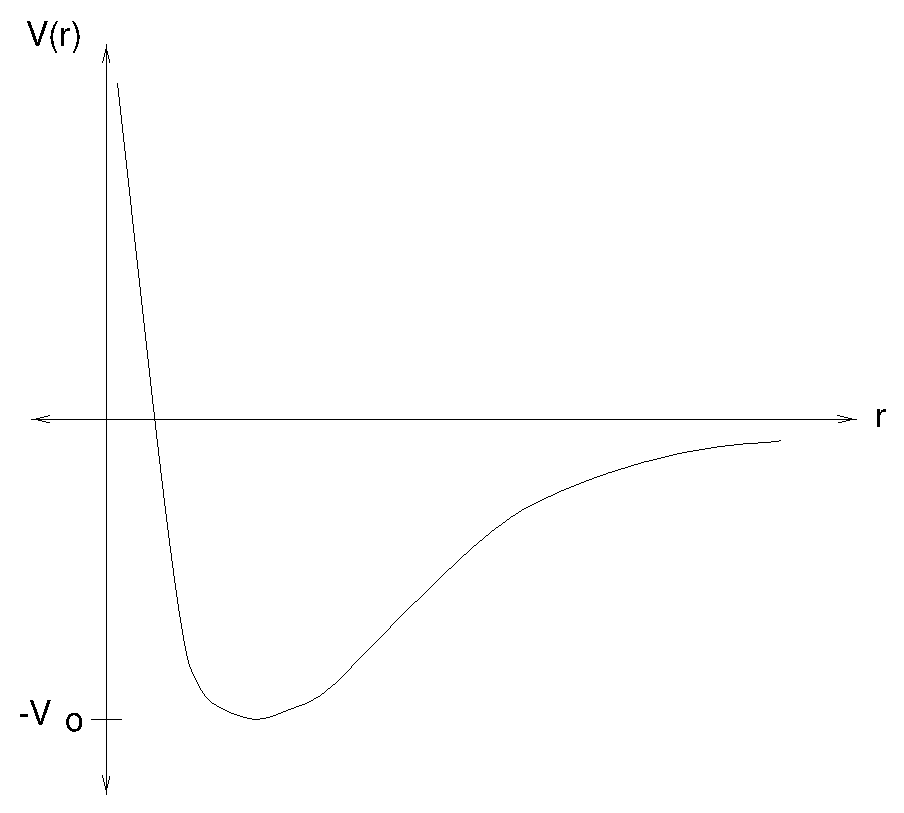
\includegraphics[height=5cm]{potential.eps}
      \end{center}

      For a quantum system such as this one, Schrodinger's Equation is
      usually used to solve for the allowed energies $E_n$ of the molecular
      system.
      \begin{equation}
       \left[ \frac{\hbar}{2m}\frac{d^2}{dr^2} + V(r) \right] = E_n\psi_n
      \end{equation}

      Due to the fact that the mass of the protons is approximated to be
      infinite, the problem can be solved using classical mechanics and
      then applying quantisation rules of the ``old'' quantum theory.

      The total energy in classical mechanics is given by the sum of the kinetic and potential
      energies.
      \begin{equation}
            E = \frac{p^2}{2m} + V(r)
      \end{equation}
      Solving for the momentum $p$ we get:
      \begin{equation}
            p(r) = \pm\sqrt{2m(E-V(r)}
      \end{equation}
      To quantize this classical motion, we consider the potential in
      phase space. The area enclosed by the phase space trajectory is
      called the ``action'' is given by $S(E)$, where $E$ is the
      energy. According the ``old'' quantum theory quantisation rules,
      for a given energy $E_n$, the action must be only half integral
      multiples of $\pi$. 

      \begin{equation}
      S(E_n) = \oint \frac{p(r)}{\hbar} dr 
      \end{equation}

      \begin{equation}
      S(E_n) = 
             2\sqrt{\frac{2m}{\hbar^2}} 
             \int_{r_{in}}^{r_{out}} \sqrt{E_n - V(r)} dr 
      \end{equation}

      \begin{equation}
      S(E_n) = 
             \left(n + \frac{1}{2} \right)\pi
      \end{equation}

      

\subsection{Aims}

    The main aim is to solve the scaled action equation, to find the quantised
    scaled energy levels $\epsilon_n$ for the different quantum levels $n$.
    \begin{equation}
        \label{main}
        s(\epsilon_n) = 
            \gamma\int_{x_{in}}^{x_{out}} [\epsilon_n - v(x)]^{1/2} dx =
            \left( n + \frac{1}{2} \right)\pi.
    \end{equation}
    The actual energy levels can then be calculated from $E = V\epsilon$.
    The aim is to solve the equation with a quadratic potential $v(x)$
    both analytically and numerically. Then the potential is to be
    replaced with the Morse potential which can only be solved
    numerically. The numerical results of the energy then need to be
    compared with the experimental results obtain for the quantised
    energy levels of the $\mathrm{H_2}$ molecule.

\subsection{Quadratic Potential Procedure}

    Using a quadratic potential $V(r)$, equation~\ref{main} needs to be solved.
    \[ V(r) = 4V_0 \left( \frac{r}{a} - 1 \right) 
                   \left( \frac{r}{a} - 2\right) \]

    We need to find the roots of $\epsilon_n - v(x) = 0$,
    $x_{in}(\epsilon_n)$ and $x_{out}(\epsilon_n)$, where 
    $x = r/a$, and $v(x) = V(x)/V_0$ and therefore $v(x) = 4(x-1)(x-2)$.
    \begin{eqnarray}
        \epsilon_n - v(x)   & = & 0 \nonumber \\
        \epsilon_n - 4(x-1)(x-2) & = & 0 \nonumber \\
        -4x^2 + 12x - 8 + \epsilon_n & = & 0 \nonumber
    \end{eqnarray}
    The roots of a quadratic are given by
    \[ x_\pm = \frac{-b \pm \sqrt{b^2 - 4ac} }{2a}\]
    \begin{eqnarray}
    x_{\pm} & = & \frac{-12 \pm \sqrt{144 + 16(\epsilon_n - 8)} }{-8} \nonumber \\
    x_{\pm} & = & \frac{-3 \pm \sqrt{\epsilon_n + 1}}{-2} \nonumber
    \end{eqnarray}
    Therefore the roots are given by:
    \[ x_- = x_{in}(\epsilon_n) = \frac{3 - \sqrt{\epsilon_n + 1} }{2} \]
    \[ x_+ = x_{out}(\epsilon_n) = \frac{3 + \sqrt{\epsilon_n + 1} }{2} \]

    With the roots of the $\epsilon_n - v(x) = 0$, know available,
    equation~\ref{main} can be solved analytically. Alternatively the
    a convenience equation can be used to solve equation~\ref{main}.
    \[ \int_{x_-}^{x_+} \sqrt{ax^2 + bx + c} dx = \frac{(4ac - b^2)\pi}{8a\sqrt{-a}} \]
    \begin{eqnarray}
        s(\epsilon_n) = \gamma\int_{x_{in}}^{x_{out}} [\epsilon_n - v(x)]^{1/2} dx & = &
                        \left( n + \frac{1}{2} \right)\pi \nonumber \\
        \gamma\int_{x_{in}}^{x_{out}} \sqrt{-4x^2 + 12x - 8 + \epsilon_n } dx & = & 
                        \left( n + \frac{1}{2} \right)\pi \nonumber \\
        \gamma\left[ \frac{4(-4)(\epsilon_n - 8) - 144}{-64} \right] & = &
                        \left( n + \frac{1}{2} \right)\pi \nonumber \\
        \gamma\left[ \frac{\epsilon_n + 1}{4} \right] & = &
                        \left( n + \frac{1}{2} \right) \nonumber \\
        \epsilon_n & = & \frac{4\left(n + \frac{1}{2}\right)}{\gamma} - 1 \nonumber
    \end{eqnarray}

    Therefore the analytic solution for the energy $\epsilon_n$ is given
    by
    \begin{equation}
    \label{quadenergy}
    \epsilon_n = \frac{4\left(n + \frac{1}{2}\right)}{\gamma} - 1 \nonumber
    \end{equation}

    Using this information, a FORTRAN program was written, to solve
    equation~\ref{main} for the quadratic potential $v(x) = 4(x-1)(x-2)$.
    The source code for the program \verb+quadratic.f+ can be found in 
    Appendix C. The program takes the quantum number n, and a value for the constant
    $\gamma$ as input.

    \begin{figure}
        \centering
        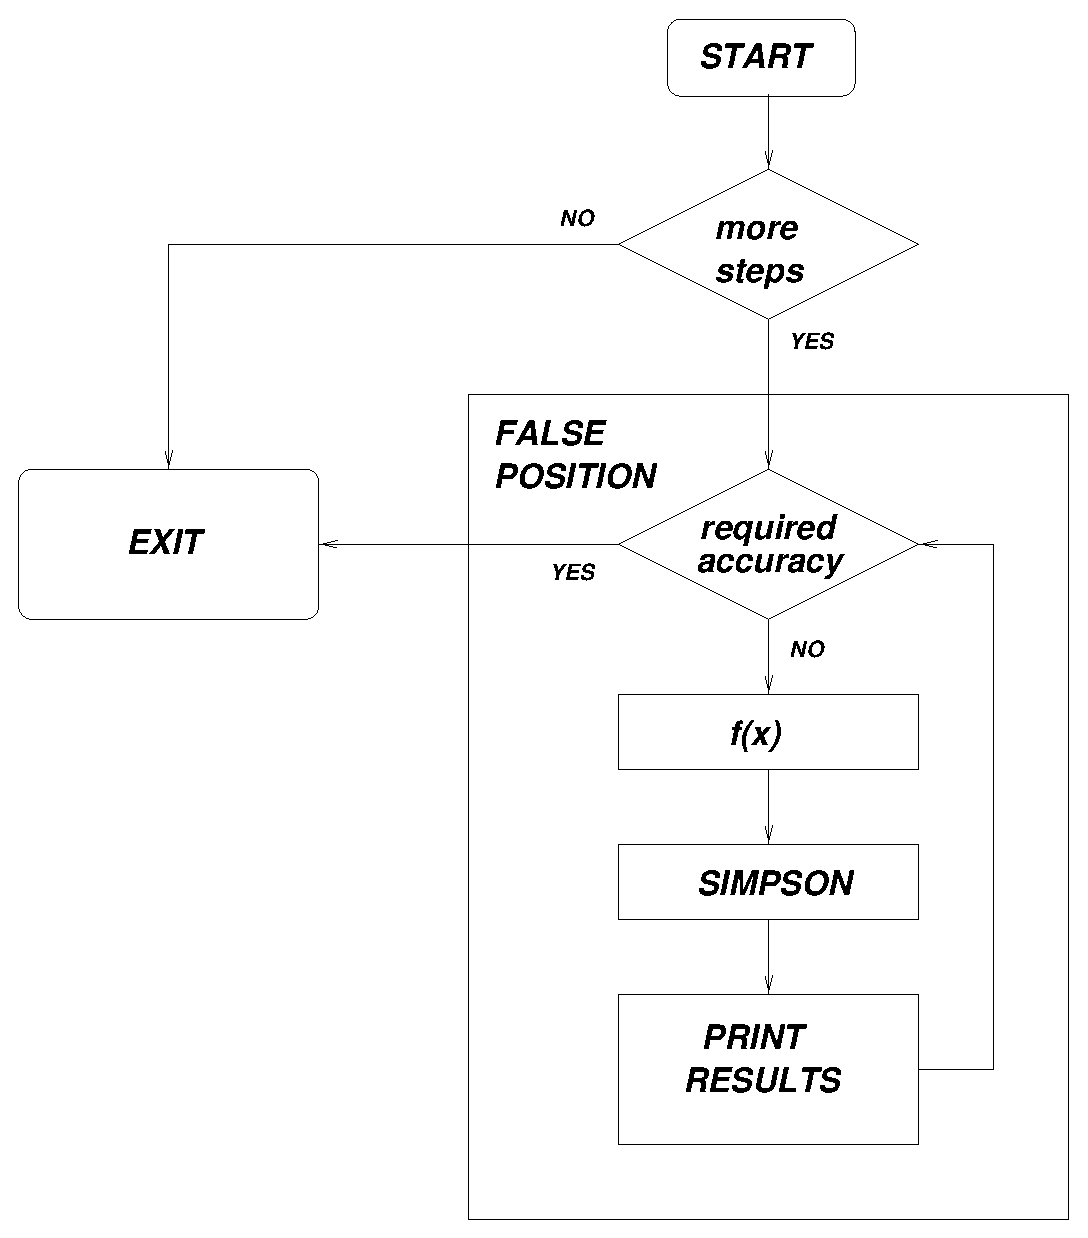
\includegraphics[width=0.8\columnwidth]{flow.eps}
        \caption{Flow chart of quadratic integration algorithm}
        \label{fig:flow-chart}
    \end{figure} 

    Figure~\ref{fig:flow-chart} shows a very high level architectural design of
    the FORTRAN program \verb+quadratic.f+ shown in Appendix C.

\subsection{Quadratic Potential Results}
    The table below shows the results of the \verb+quad.f+ program for
    the values of $n = 0,1,2,3,4$, and with $\gamma = 1$. Since the
    accuracy of this method was investigated for different step sizes
    and tolerance values in the previous section, the results here all
    have $10^6$ divisions for Simpson's rule and a tolerance of
    $10^{-6}$ for the false position algorithm.
  
    The column labelled $\epsilon_n$ is the analytic solution to
    equation~\ref{main} for $v(x)$ given by equation~\ref{quadenergy},
    whereas the column labelled $\epsilon_n^{*}$ is the solution given
    by the FORTRAN program \verb+quadratic.f+.

    \begin{table}[h] 
    \caption{Values of $\epsilon_n$ for a quadratic potential with $\gamma = 1$.}
    \label{tbl:epsilon} 
    \begin{center}
    \begin{tabular}{|r|r|c|c|} \hline
    $n$ & $\epsilon_n$ & $\epsilon_n^{*}$ & $Error$ \\ 
    \hline
    \hline
    0   &   1   &   1.0000000008    &   .826897E-09 \\ 
    1   &   5   &   5.0000000025    &   .248070E-08 \\ 
    2   &   9   &   9.0000000041    &   .413422E-08 \\ 
    3   &  13   &  13.0000000058    &   .578873E-08 \\   
    4   &  17   &  17.0000000074    &   .744295E-08 \\ \hline
    \end{tabular}
    \end{center}
    \end{table} 

    To look at the numerical stability of the program, we vary the
    number of divisions $N$ in the Simpson quadrature algorithm, and the
    tolerance in the false position algorithm. Taking just one of the
    values of $n$, we have the following results for $n = 1$ and
    $\gamma = 1$, in the table below.

    \begin{table}[h]
    \caption{$\epsilon_n$ for $n=1$, $\gamma = 1$,
                    for varying tolerances for quadrature and root
                    finding algorithms.  }
    \label{tbl:epsilon-prime} 
    \begin{center}
    \begin{tabular}{|r|r|c|c|} \hline
    $N$ & $Tolerance$ & $\epsilon_n$ & $Error$  \\
    \hline
    \hline
              10 &.1000000  &5.0801607150   &.801607E-01 \\
             100 &.0100000  &5.0024839897   &.248399E-02 \\
            1000 &.0010000  &5.0000784582   &.784582E-04 \\
           10000 &.0001000  &5.0000024808   &.248084E-05 \\
          100000 &.0000100  &5.0000000785   &.784505E-07 \\
         1000000 &.0000010  &5.0000000025   &.248070E-08 \\ \hline
    \end{tabular}
    \end{center}
    \end{table} 


\subsection{Quadratic Potential Discussion}

    Looking at Table~\ref{tbl:epsilon}, we see good agreement with the values calculated
    analytically for $\epsilon_n$ and those calculated numerically, with 
    an error of approximately $10^{-8}$ for all cases except for when
    the $n = 0$, when the error is approximately $10^{-9}$. 
    The technique can then be used solve the problem of finding the
    quantized energy levels with more complicated and more physically
    realistic potentials such as the Morse potential, which there exists
    no analytic solution and must therefore be solved numberically.

    Looking at Table~\ref{tbl:epsilon-prime}, we see the results for varying tolerances for
    both the quadrature (Simpson's) algorithm, $N$, and the root finding
    algorithm (false position), $Tolerance$, for $n=1$ and $\gamma=1$.
    We see that the algorithms used result in numerically stable
    solutions by oberving that the error consistently decreases, as $N$
    is increased and as the $Tolerance$ is decreased.
    

\subsection{Morse Potential Procedure}

      The procedure was to modify the program used to calculate
      $\epsilon_n$ from using a quadratic potential, to a potential that
      was closer in shape to what had been observed in experiments.
      This is the Morse potential given by
      \begin{equation}
      V_{Morse}(r) = V_0\left[\left(1-e^{-(r-r_{min})/a}\right)^2 - 1\right]
      \end{equation}
      The Morse potential can be normalised ($x=r/a$ and $v(x)=V(r)/V_0$)
      to get
      \begin{equation}
            v(x) = \left( 1 - e^{-(x-x_{min})} \right)^2 - 1
      \end{equation}
      The next step is to analytically find the turning points
      $x_{in}(\epsilon_n)$ and $x_{out}(\epsilon_n)$ of the 
      equation $\epsilon_n - v(x) = 0$.
      \[ \epsilon_n - \left[ \left( 1 - e^{-(x-x_{min})} \right)^2 - 1 \right] 
                                                 =  0 \]
      Let $z = e^{-(x - x_{min})}$
      \begin{eqnarray}
            \epsilon_n - [ (1-z)^2 - 1] & = & 0\nonumber \\
            \epsilon_n - (z^2 - 2z) & = & 0 \nonumber \\
            z^2 - 2z - \epsilon_n & = & 0 \nonumber
      \end{eqnarray}
      Solve for z using
      \begin{eqnarray}
       z_\pm & = & \frac{-b \pm \sqrt{b^2 - 4ac} }{2a} \nonumber \\
       z_\pm & = & \frac{2 \pm \sqrt{4 - 4(1)(-\epsilon_n)} }{2} \nonumber \\
       z_\pm & = & 1 \pm \sqrt{1 + \epsilon_n} \nonumber
      \end{eqnarray}
      Now substitute $z$ back in to get
      \begin{eqnarray}
            e^{-(x_{\pm} - x_{min})} & = & 1 \pm \sqrt{1 + \epsilon_n} \nonumber \\
            -(x_{\pm} - x_{min}) & = & 
                        \ln\left(1 \pm \sqrt{1 + \epsilon_n}\right) \nonumber\\
            x_{\pm} & = & x_{min} - 
                  \ln \left( 1  \pm \sqrt{1+\epsilon_n} \right) \nonumber
      \end{eqnarray}
      Therefore $x_{in}(\epsilon_n) = x_{min} - \ln(1 + \sqrt{1-\epsilon_n})$ and
      $x_{out}(\epsilon_n) = x_{min} - \ln(1 + \sqrt{1+\epsilon_n})$.

      The following procedure was then followed:
      \begin{itemize}
            \item The \verb+quadratic.f+ program was modified to change
                  the potential from quadratic to Morse and to add the
                  new turning points calculated above.
            \item The source code for the new program \verb+morse.f+ can
                  be found in Appendix D.
            \item For the case of $n=0$, the program was run with a
                  number of different values of a, until a value was
                  found such that the value given for the energy
                  $E_n = V_0\epsilon_n$ was very close to value of
                  $E_0 = -4.477$ as given in Table 1.5 of Koonin
                  (experimental result).
            \item Using the final value of $a$, the first four quantised
                  energy levels were calculated with the program and
                  compared with the experimental results for the
                  $\mathrm{H_2}$ spectrum.
            \item The choice of starting values for $\epsilon_n$, is
                  restricted by the turning points, \\
                  $x_{\pm}  =  x_{min} - 
                  \ln \left( 1  \pm \sqrt{1+\epsilon_n} \right)$.
                  We can see from this equation that 
                  $-2 < \epsilon_n \le 1$.
      \end{itemize}

\subsection{Morse Potential Results}

      \subsubsection{Determining the parameter $\mathbf{a}$}
      The table below shows the results of inputing different values of
      $a$ into the \verb+morse.f+ program. We have the following values:
      \begin{itemize}
            \item $\gamma = 33.6567a$
            \item $r_{min} = 0.74166 \: \mathrm{\dot{A}}$, 
                  $x_{min} = 0.74166a \: \mathrm{\dot{A}}$
            \item $V_0 = 4.747 \: \mathrm{eV}$, $(E_n = V_0\epsilon_n)$
            \item $n = 0$
            \item $N = 1000$ (Number of divisions in Simpson's Rule)
            \item $T = 10_{-3}$ (Tolerance in false position method)
      \end{itemize}
      From experimental results looking at the spectrum of the Hydrogen
      molecule, we know that for the lowest energy state (when $n=0$),
      we have $E_0 = -4.477 \: \mathrm{eV}$. Therefore, for a given
      value of $a$, we are looking for 
      $\epsilon_0 = -4.477/4.747 \simeq -0.943121971$.

      \begin{table}[h] 
      \caption{Values of $\epsilon_0$ for different values of the parameter $a$.}
      \label{tbl:epsilon-zero} 
      \begin{center}
      \begin{tabular}{|c|c|} \hline
      $a$ & $\epsilon_0$ \\ \hline \hline
      0.50  &     -.9414586271  \\
      0.60  &     -.9510928378  \\
      0.55  &     -.9467075966  \\
      0.52  &     -.9436775546  \\   
      0.51  &     -.9425895401  \\ 
      0.515 &     -.9431387536  \\ \hline 
      \end{tabular}
      \end{center}
      \end{table} 

      We see from Table~\ref{tbl:epsilon-zero} that we get closest to the value of
      $\epsilon_0$ when $a = 0.515$.

      Using this value of $a$, we can then run the program for the first
      4 values of $n = 0,1,2,3$ and compare to the experimental results.
      Since the experimental results are only available to 3 decimal
      places, it is meaningless to attempt to calculate solutions with
      more accuracy since we don't have more accurate experimental data
      to compare with. In all cases the calculations were done with 1000
      divisions in Simpson's rule and a tolerance of $10^{-3}$ for the
      root finding false position algorithm.

      The results of the running the program for the first four energy
      levels are shown in Table~\ref{tbl:first-four}, where $E_n^{*}$ is the
      numerical result calculated using the program and $E_n$ is the 
      experimental result from Table 1.5 of Koonin.

      \begin{table}[h]
      \caption{First four quantized energy levels of
      the spectrum of the $H_2$ molecule.}
      \label{tbl:first-four} 
      \begin{center}
      \begin{tabular}{|c|c|c|c|c|} \hline
      $n$   &   $\epsilon_n$  & $E_n^{*}$       &  $E_n$    & $Error$   \\\hline \hline
      0     &   -.9431387536  & -4.4770796631   & -4.477    & .796631E-04 \\
      1     &   -.8344090650  & -3.9609398314   & -3.962    & .106017E-02 \\ 
      2     &   -.7323362062  & -3.4763999710   & -3.475    & .139997E-02 \\
      3     &   -.6369210780  & -3.0234643571   & -3.017    & .646436E-02 \\ \hline
      \end{tabular}
      \end{center}
      \end{table} 

\subsection{Morse Potential Discussion}

      As can be seen from Table 7, the values of the energy levels of
      the Hydrogen molecule for quantum levels $n = 0,1,2,3$, have a
      good agreement with the experimental results. The error was of
      magnitude $10_{-2}$ for $n = 1,2,3$ and of magnitude $10_{-4}$ for
      $n = 0$. 

      The agreement between calculation and experiment is good,
      especially considering the use of the old quantum theory in the
      numerical calculations.

      More insight could have been gained into the accuracy of the
      numerical techniques used to do the calculations if the
      experimental data presented for the Hydrogen molecule spectrum was
      more accurate.

      With all the data now available we can make a plot of the equation
      \[ V_{Morse}(r) = V_0\left[\left(1-e^{-(r-r_{min})/a}\right)^2 - 1\right]. \]
      Using the values for $\gamma$, $a$, $r_{min}$, and $V_0$, shown in
      the previous section we can plot the Morse potential for the
      Hydrogren molecule in Figure~\ref{fig:morse} 

        \begin{figure}
        \centering
        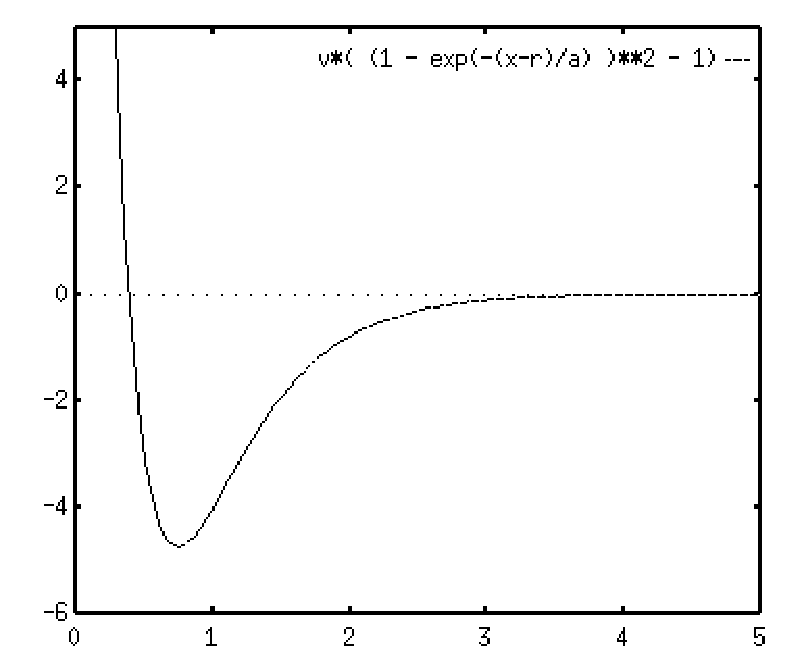
\includegraphics[width=0.8\columnwidth]{morse.eps}
        \caption{Morse Potential for Hydrogen Molecule} 
        \label{fig:morse} 
        \end{figure} 


      Using the data for the first four quantized energy levels, we can
      plot these on top of the Morse potential plot, shown in 
      Figure~\ref{fig:levels}. 

        \begin{figure}[ht] 
        \centering
        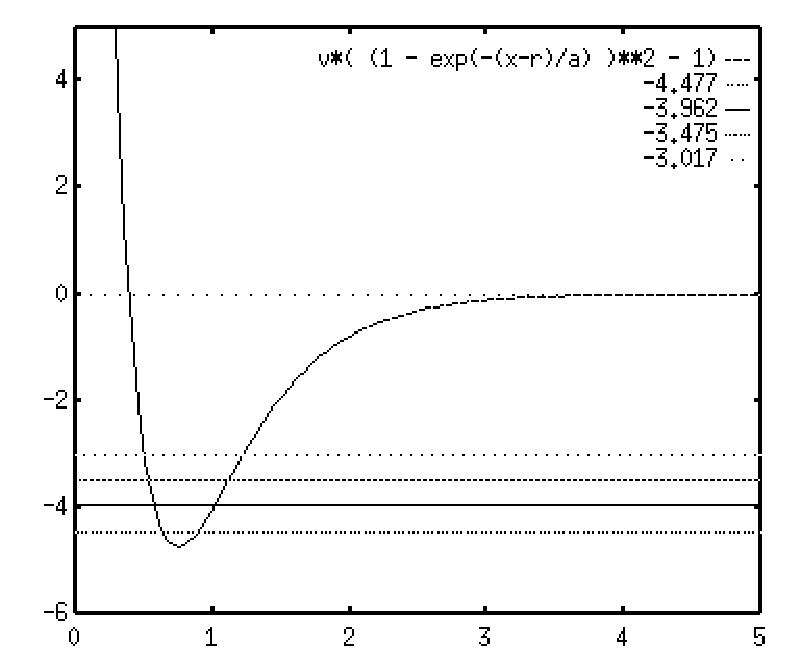
\includegraphics[width=0.8\columnwidth]{levels.eps} 
        \caption{First Four Quantized Energy Levels} 
        \label{fig:levels} 
        \end{figure} 


%----------------------------------------------------------------------
% APPENDICES
%----------------------------------------------------------------------

\onecolumn

\appendix[Code Listing: quad.f]
\showcode{quad.f} 

\newpage 
\appendix[Code Listing: root.f] 
\showcode{root.f} 

\newpage 
\appendix[Code Listing: quadratic.f] 
\showcode{quadratic.f}

\newpage 
\appendix[Code Listing: morse.f] 
\showcode{morse.f}

%----------------------------------------------------------------------
% END DOCUMENT
%----------------------------------------------------------------------

\end{document}

%----------------------------------------------------------------------
